	\chapter{Software}
		This chapter provides information about the software located on \index{BaralabaBob}BaralabaBob's controller, and required to run and program it.
		\pagebreak
	
		\section{Operating System}
			I'm currently running \index{Raspbian}\index{Linux}\index{Deebian}Raspbian. Raspbian is a distribution of Debian linux compiled specifically for the ARM based instruction set of the Raspberry Pi. Experimentation has been done with Arch Linux to no end.
		
			\subsection{Image Download}
            	\index{image}
                \index{ISO}
                \index{Rasberry Pi}
                \index{RPi}
				Currently I have no pre-made image ready for download. This will hopefully change in time. I could simply read the SD card and save the ISO to my website - but pratically the ISO will be 32GB. A better option is to set up some system which reads the currently used disk and saves that to an ISO on the actual RPi - but I haven't set that up yet.
				
               	\index{Win32DiskImager}
				This image can be restored to the SD card using a program such as Win32DiskImager. I decided to go down the path of imaging the SD card because I was frequently having to rebuild the entire OS when something corrupted (when I was using cheap SD cards). Although I am no longer using cheap SD cards, I consider it good practice to keep a good base image of the OS ready to go if anything happens.
	
	
			\subsection{Building Image}
            \index{Raspbian}
            \index{install}
            \index{configuration}
            \label{raspbian_install}
				\begin{itemize}
					\item Raspbian image should be downloaded from \url{http://www.raspberrypi.org/downloads/}. Torrenting is a good option for downloading for speed.
					\item Write the image to an \textit{MicroSD Card} of a size no smaller than 8GB using Win32DiskImager.
					\item Edit cmdline.txt to remove all references to a serial console. (The reason for this is because I'm using the UART line on the RPi to communicate with the SCC-32 servo controller, and whilst booting the serial console sends invalid command signals to the SCC-32.)
					\item Plug in ethernet cable to the RPi and a DHCP enabled switch/router/server.
					\item Use Advanced Port Scanner (From Radmin) to scan the network for new IPs/IPs with the manufacturer ID of Raspberry Pi Foundation.
					\item Log in using SSH (use PuTTY on Windows, ssh command from terminal on *nix systems). Default username and password are pi and raspberry respectively.
					\item Run \textit{"rm -rf python\_games"} (This cleans up the home directory from unnecessary clutter).
					\item Run \textit{"sudo raspi-config"}
					\item Select "expand filesystem".
					\item Reboot.
					\item Relog into SSH.
					\item Run \textit{"sudo apt-get upgrade"}
					\item Run \textit{"wget --user=[MY BITBUCKET USERNAME] --password=[MY BITBUCKET PASSWORD] https://goo.gl/QlJj7C"} (This downloads a script which will download the required packages.)
					\item Run \textit{"sh setup\_pi.sh"}. Fill in required information as required! The git clone from GitHub will fail as the repository is no longer located there. Will fix up this issue some time.
					\item Add "UseDNS no" to the end of \textit{/etc/ssh/sshd\_config}. This disables DNS reverse lookup.
					\item In the future there will be instructions on how to install the RPi drivers for the new AWUS036NHV WiFi module.
					\item No need to git clone any repositories onto the device, as repository is installed on my computer, and uploaded using the remote deployment feature in Pycharm, which uploads all files to the RPi.
					
				\end{itemize}
			
		
		\section{Networking}
        	\index{networking}
        	\label{rpi_networking}
			The primary mode of communication with the RPi to program it and monitor it's state is through the network interface(s). This section outlines the configuration of those interfaces.
			
			\subsection{Ethernet}
            	\index{ethernet}
				The RPi has a static IP configured for eth0 on 192.168.2.100. Configure your computer’s Ethernet interface to 192.168.2.1, and proceed to login over SSH.
				
			\subsection{WiFi}
            	\index{WiFi}
				In the future the RPi will create an ad-hoc network, and enable DHCP, allowing people to login using specified credentials.
				
			\subsection{Serial}
            	\index{serial}
                \index{RS-232}
                \index{UART}
				A network interface can be configured to use the serial terminal, however this has not been enabled on the BaralabaBob as the serial line is being used to control the SCC-32 Servo Controller.
	
			\subsection{Current Configuration}
            	\index{configuration}
                \index{install}
                \index{IP address}
				Network configuration is located in \emph{/etc/network/interfaces} in Raspbian.\\
			
				\begin{lstlisting}[frame=single]
auto lo
iface lo inet loopback

iface eth0 inet static
address 192.168.2.100
netmask 255.255.255.0
gateway 192.168.2.1

auto wlan0
allow-hotplug wlan0
iface wlan0 inet static
address 192.168.0.8
netmask 255.255.255.0
gateway 192.168.0.1

wpa-ssid "BigPond3BF6"
wpa-psk  "<BigPond3BF6 Password>"
				\end{lstlisting}
				\pagebreak
	
	
		\section{Access}
        	\index{login}
            \index{ssh}
            \index{terminal}
			There are three options for accessing the RPi’s terminal. The most common, and the one we will be using throughout this manual is SSH over a network interface.\\
			
			When logging in, use the username “pi” and the specified password.\\
		
			\subsection{Terminal}
				Terminal access gives access to the linux terminal.
		
			\subsubsection{SSH}
				Using an SSH program (Putty on Windows and ssh in the terminal of Mac and Linux machines), you can connect to the RPi over one of its network interfaces. For reasonably fool-proof testing, Ethernet is the most reliable.
		
				\subsubsection{Physical}
					This is the most fool-proof way to access the terminal. It involves plugging in a monitor using the RCA or HDMI ports, and plugging a keyboard over USB. One gotcha is if the monitor is not properly configured. If this is the case, remove the SD card from the RPi, plug it into a computer, and edit the config for your particular monitor option.
					
				\subsubsection{Serial}
					A default Raspbian install provides by default a serial on the terminal port. This, however, has been disabled to allow communication over that serial port to the SCC-32 Servo Controller. Having the serial terminal enabled while the SCC-32 Servo Controller is powered will cause the servos to go haywire.
					
			\subsection{File}
            	\index{file access}
                \index{FTP}
				File access provides the ability to transfers to and from the controller.
				
				\subsubsection{SFTP}
					File access is available over SFTP (using SSH). FileZilla (for Windows) has the ability to connect to it. Make sure to use Port 22 (the SSH port) when connecting in FileZilla.
					
				\subsubsection{FTP}
					VSFTPD has been installed in the past, however has been replaced with SFTP for the sake of removing unrequired software. Consequence of this is that the pi is no longer accessible directly from Windows Explorer, and needs external software, such as FileZilla when connecting over SFTP (see above).
		
	\pagebreak
	
		\section{Software Used}
        	\index{software}
			This is a list of the software used in the development of this robot. All software is aimed for someone using a windows machine. All software mentioned below is available for download directly off the Pi. See Embedded Downloadable Resources for more.
		
			\subsection{Blender}
            	\index{Blender}
				Blender is open source 3D animation, modelling, game making, etc software. It is written in python and contains an excellent API and scripting interface allowing me to code addons allowing easy interfacing between the robot and Blender. Using Autodesk Maya was considered in place of Blender, however due to its cost, size, availability, and closed source nature, I opted for Blender. More on this later ;D\\
				
				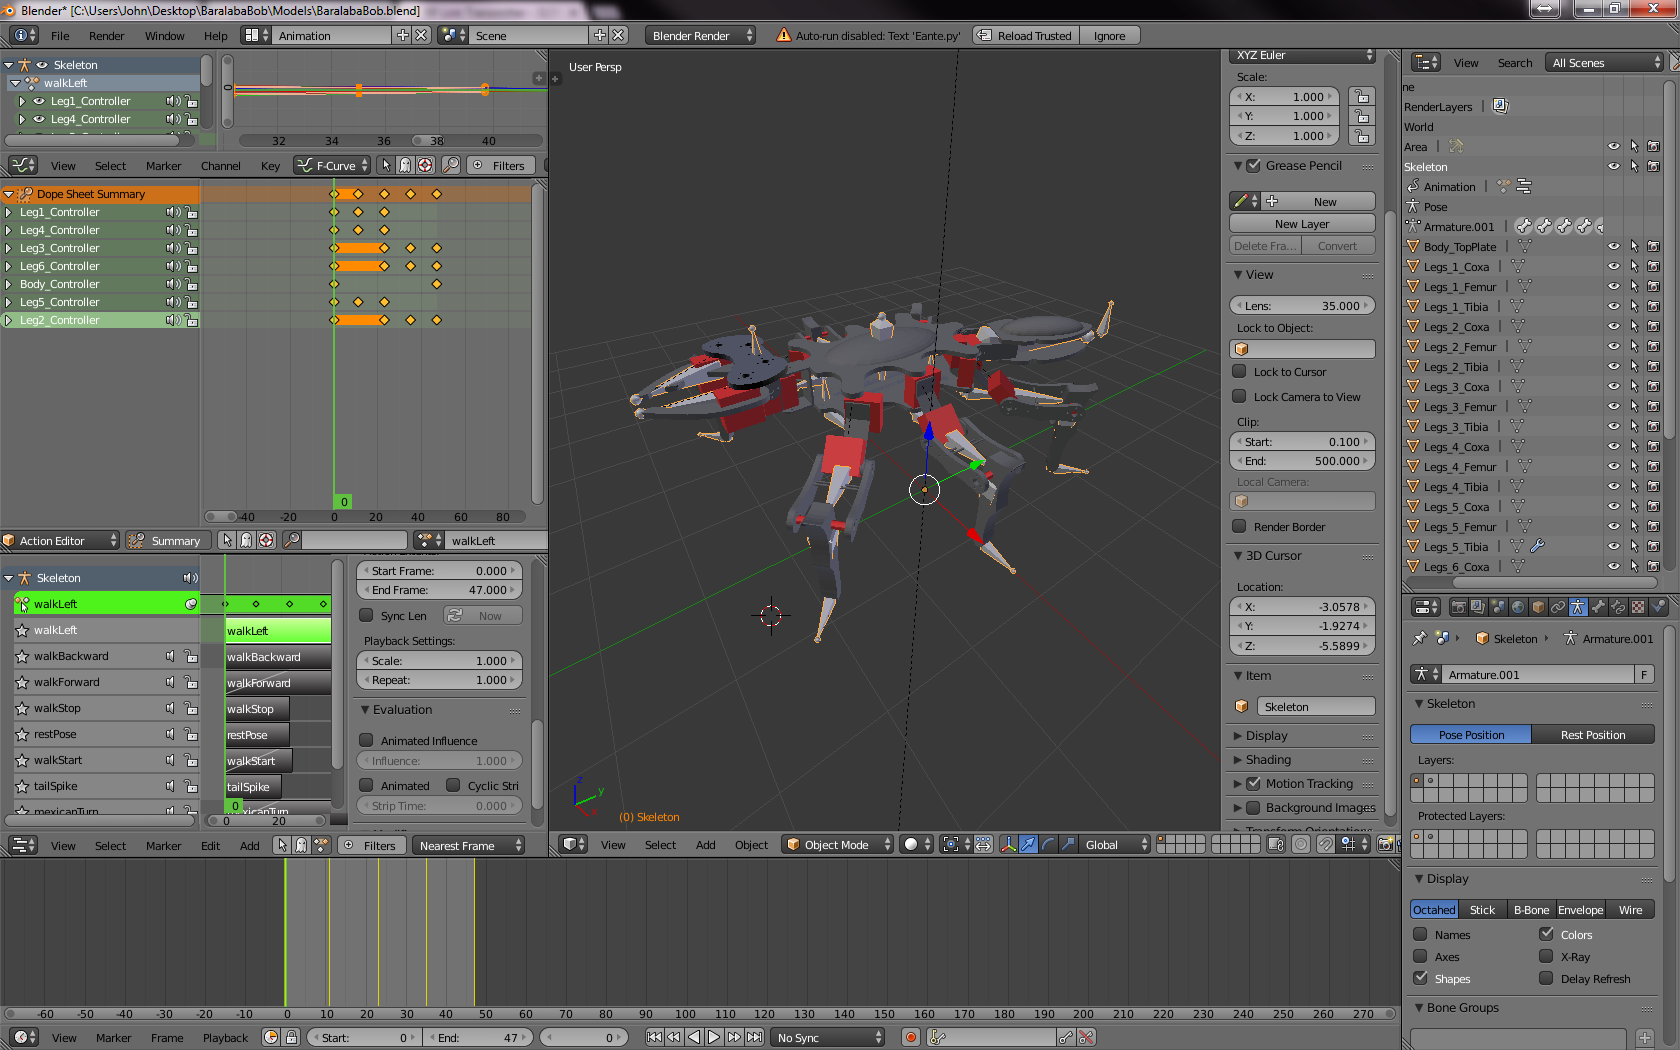
\includegraphics[width=\linewidth]{blender}
			
			\subsection{PuTTY}
            	\index{PuTTY}
                \index{SSH}
				Putty is a lightweight program that I use for accessing the SSH terminal on the RPi.
				
			\subsection{PyCharm}
            	\index{python}
                \index{PyCharm}
				PyCharm is my preferred python editor which I use for programming the python code on the robot. There is a freely available community version. Alternately you can access a student version freely for a year if you have a student email address. I’ve done the latter, and as such can access a full version of PyCharm until March 2016.\\
				
				The main advantage of the full version is that it is able to remotely edit code using SFTP, and remotely execute code using SSH. This is really advantageous for this purpose.
				
			\subsection{Python 3.4.3}
            	\index{python}
				The python runtime is required for the running of the code. We are using Python 3.4.3 as the standard version across the board if at all possible.
			
			\subsection{FileZilla}
            	\index{FTP}
                \index{FileZilla}
				Filezilla is a program for accessing a FTP/SFTP server. It is used for accessing the SFTP server on BaralabaBob.
				\pagebreak
			
	
		\section{Blender}
        \label{manual_blender}
        \index{Blender}
		BaralabaBob uses a custom version of Blender. The differences are listed below:
		
			\begin{itemize}
				\item RPyC Included
				\item \textbf{TODO: Script/ADDON Included}
			\end{itemize}
			
			At the time of writing, the version was 0.1.					
	
			\subsection{Building Blender Image}
            	\index{blender image creation}
				BaralabaBob uses a "custom" version of blender. Custom in the sense that I've added python libraries to a .zip distribution. This version of blender is also in a portable form - no install is required. It's based off a 32-bit built of Blender 1.73a. Downloaded 24/03/2015.
							
				\begin{itemize}
					\item Downloaded 32-bit zip for windows from \emph{\url{http://blender.org/download/}}
					\item Extract the .zip
					\item Download .zip source of RPyC \emph{\url{https://pypi.python.org/pypi/rpyc}}
					\item Extract that .zip
					\item Navigate to blender\_folder\textbackslash 2.73\textbackslash python\textbackslash lib\textbackslash site-packages\textbackslash
					\item Install the RPyC source folder into site-packages
					\item \textbf{NOTE: Install scripts coming...}
					\item Upload to website, under robotics folder.
				\end{itemize}
				
				\pagebreak
	
	
		\section{Embedded Content}
        	\index{embedded content}
            \index{download-able content}
			The pi hosts a website accessible from the local network which contains the files for all programs required.\\
			
			\textbf{Location:} \url{http://<pi_network_location>/files/}\\
			
			For example, \url{http://192.168.2.100/files}
			\pagebreak



	\chapter{Programming}
    	\index{programming}
		The \index{BaralabaBob}BaralabaBob project as a whole has had significant time put into the programming of it.
		
		There are two main divisions of the code - Frontend, and Backend. \\
		
		\index{backend}Backend software generally is directly to do with actually moving the robot around in it's enviroment. Amelior, Shalom, and GoombungeeShowClient all would be conisidered backend projects.\\
		
		\index{frontend}Frontend is software that allows human interaction with the robot. This software includes Eante.py and Dumper.py, GoombungeeShowServer, IK Experiment, and JoystickController. Eante and Dumper are directly related to the animation cycle of the robot, whereas JoystickController is to do with real-time remote control of the robot.\\
		\pagebreak

		\section{Backend}
        	\index{backend}

			\subsection{Amelior}
            	\index{Amelior}
				\label{Amelior}
				\begin{quote}
					\textit{\textbf{Ameliorant}, verb} - to make or 			become better.
				\end{quote}
			
				Amelior comprises of what used to be the \hyperref[BaralabaBob]{BaralabaBob} module in the Goombungee Exhibition days. Amelior contains the base, "object oriented" model for the robot, including event system, and blender animation playback functions. Experimental inverse kinematics mode has been added, with promising results.\\
			
				\subsubsection{Model}
                	\index{model}
					There are two forms of "Model" referred to in the Amelior project. One is purely mathematical, in the form dimensions and positions, outlined in configuration files. The other "model" is an object-based one, being composed of python classes.\\
					
                    \index{mathematical model}
					\textbf{Mathematical} - This comprises of several configuration files outlining the demensions and positions of relevant mechanical systems on BaralabaBob. These configuration files were designed to be easily "swap-outable", allowing this codebase to work on several different hexapod platforms, with the corresponding configuration files.\\
					
					These files can be found under \textit{BaralabaBob/Codebase/Amelior/config/model/BaralabaBob/}. \\
					
                    \index{objective model}
					\textbf{Objective} - this comprises of several pythonical objects forming a model. Through modifying variables and calling functions this model can be manipulated. The top object is considered the "Hexapod" object, giving system-wide commands like "turnOn" and "turnOff". Hexapod has sub-objects of legs, mandibles, and tail. Legs has sub objects of 6 instances of the leg object. \\
					
					At the mandibles, tail, and leg object levels there are several "joint" objects. Each joint represents a physical motor in reality. For the legs there are 3 joint objects, the coxa (hip), femur (upper-leg), and tibia (lower leg).		\\
					
				\subsubsection{Scripting}
                	\index{scripting}
					In the early days of BaralabaBob I needed a way to program routines into the robot. I decided that writing python "scripts" was the best way to go.\\
					
					The scripts can be found in the \textit{BaralabaBob/Codebase/Amelior/config/model/BaralabaBob/scripts/} directory.\\
					
					The "script executor" (actually named sequence executor) is located at \textit{BaralabaBob/Codebase/Amelior/util/scriptexecutor.py}.\\
					
					The script executor code could either import a local script, or even download one over HTTP, and then execute it. The script executor was controversially named "sequenceexecutor" - which later clashed with the Blender Playback code, which was then named script-executor. This problem has yet to be rectified.
						
				\subsubsection{Blender Playback}	
                	\index{blender playback}
                    \index{scripting}
                    \index{ACT files}
                    \index{actions}
                    \index{keyframe}
					As outlined in the Blender section, I developed code that would plug into blender and would export animation data, for later playback on the robot.\\
					
					Both the scriptexecutor.py and action.py located in the \textit{BaralabaBob/Codebase/Amelior/util} folder open and can playback  any seqeunces located in the \textit{BaralabaBob/Codebase/Amelior/config/model/BaralabaBob/actions/} folder. \\
				
					The average .act file includes information including the name of the sequence, the number of frames, and keyframe information.\\
					
					The keyframe section of an .act file includes information for each keyframe in the animation, along with the where the joints have to be at that keyframe.\\
					
					Keep in mind that the joints have to be at that position by the time that keyframe gets reached. For example, if I'm at Frame 0, and Leg1.Tibia needs to be at angle 30 by frame 72, I'll move it 10 degrees per second for 3 seconds, when the framerate is 24 fps.\\
					
					When I issue a command for an action to be played back, action.py starts a while loop. Inside that while loop there is a "time checker". The "time checker" checks the time since the start of the animation, and then tells certain frames to play when their time has arrived.\\
					
					Because of the way this code is structured, if the process is running slow, it may skip a frame. Although unlikely that it would skip a frame, it does so to ensure timing with the music is maintained (in the case of a RoboCup Dance performance).\\
				
					\textbf{Also see: }\hyperref[Blender]{Blender}
							
				\subsubsection{Inverse Kinematics}
                	\index{inverse kinematics}
					Inverse Kinematic tells a system at what angles the joints should be for the end of an arm/leg to be at a certain position in a multi-jointed arm/leg.\\
					
					In the case of this \index{hexapod}hexapod I need to be able to tell the robot to move the foot to certain position, and it figure out in real time what joints to move, and where, to achieve that. This feature has been implemented, and is working solidly.\\
					
					Another feature of the Inverse Kinematics should be that I can move the base of the body, whilst the legs stay in place. Because this is modifying the positions of the "leg chain" in the opposite direction to normal, it's a little more difficult to implement. This code works, but is in experimental status.\\
					
					A fully fledged IK system would allow me to tell a robot to move (for example) to 20cm, 20cm (X, Y), and it would figure out all the steps it needs to take to get there, and then executes that. This again is in experimental status.\\
				
					It can be found under \textit{/BaralabaBob/Codebase/Amelior/} in the \hyperref[Repository]{repository}.\\

			\subsection{Shalom}
            	\index{shalom}
				\begin{quote}
					\textit{\textbf{Shalom}, interjection} - Peace, to be at peace. To be harmonious.
				\end{quote}
				
				Shalom is my first attempt at combining Inverse Kinematics with a hexapod model. I envision a much smoother and harmonious coexistance between the code and the machine with repository as it's calculating the moves on the fly, rather than following some preprogrammed routine.\\
				
				Development of this project has somewhat died due to the time it would take to rewrite a fairly decent system, that is the \hyperref[Amelior]{Amelior} project. This project was meant to contain the Inverse Kinematics code, however I ended up implementing a trial version of it in the Amelior code.\\
				
				It can be found under \textit{/BaralabaBob/Codebase/Shalom/} in the repository.\\

			\subsection{BaralabaBob}
				\label{BaralabaBob}
               	\index{BaralabaBob}
				BaralabaBob was the original "Operating System" code for the Hexapod. It contained a "object-oriented" model of the hexapod. By manipulating the objects in the model, it would send an event call through the system which would in turn send data to the servo controllers.\\
				
				This code was designed to be specific to BaralabaBob, and could not be used on other platforms. It was also designed to specifically link in with the GoombungeeShowServer/Client software, allowing the robot to be controlled by a smartphone as part of an exhibit.\\
				
				
				BaralabaBob was superceeded by \hyperref[Amelior]{Amelior}. According to the online \hyperref[Repository]{repository} this merge/shift happened on the 12th of March, 2015. The commit code is  \href{https://bitbucket.org/boar401s2/baralababob/src/441d5788267d?at=master}{441d578}. Around this time the repository was shifted from GitHub to BitBucket. The repository titled BaralabaBob originally housed only the Operating System code, the code was renamed to Amelior, and other projects were also put in the repository.

			\subsection{GoombungeShowServer}
				This code was written to connect the Javascript frontend (as seen in GoombungeeShowClient) with the python backend of Amelior (or what was BaralabaBob)\\
				
				It can be found under \textit{/BaralabaBob/Codebase/GoombungeeShowServer/} in the repository.

			\subsection{GoombungeeShowClient}
				This code was written to provide a way for people to control the robot using their phone by connecting to a website (contained in this code).\\
				
				\textit{NOTE: } My IDE of choice for editing the JavaScript was KomodoEdit\\
				
				It can be found under \textit{/BaralabaBob/Codebase/GoombungeeShowClient/} in the repository.

			\subsection{IKExperiment}
			This code I wrote when I was first playing around with the IK algorithms. It features a pygame frontend to allow you to see visually the results in real time.\\
			
			It can be found under \textit{/BaralabaBob/Codebase/IKExperiment/} in the repository.\\

			\subsection{JoystickController}
			This code is used to control the robot using a joystick.\\
			
			It can be found under \textit{/BaralabaBob/Codebase/JoystickController/} in the repository.\\
			\pagebreak

		\section{Blender}
			\label{Blender}
            \index{Blender}
			Blender is the primary method of programming the robot. Michael Board created a model of the Lynxmotion A-Pod in TurboCad 11, and exported it as 3DS format. It was then imported into Blender and rigged by John Board.\\
			
			In the early days of BaralabaBob, I realized assumed that I didn't have the nouse to write the inverse kinematics code, and I also knew that creating any kind of good hexapod routine would be difficult with textual commands - so I seeked an alternative.\\
			
			Several years previously I had developed a theoredical idea for a software which would allow you to animate a robot in 3D animation software, such as Blender or Autodesk Maya, export that animation data, and then play it back on the robot.\\
			
			I whittled my options down to Blender or Maya because of both of their abilities to have scripts written in python for them, making it easily compatible with the rest of the system. (Also my affinity with python may have biased my decision slightly...)

			\subsection{Location}
            	\index{blender location}
				Under the git repository, the models loc Thd: \emph{/root/Models/Boilerplate.} The Boilerplate template is a file which does not change, and can be considered a solid foundation for future experimentation and routines.
			
			\subsection{Blender Design Standards}
            	\index{design standards}
				The leg joints all conform to three basic joints:
			
				\begin{itemize}
					\item When Coxa joints move towards the front 		of the robot, their angles become more 				positive.
					\item When Femur joints move upwards, their 		angles become more positive.
					\item When Tibia joints move outwards, their 		angles become more positive.
				\end{itemize}
				\pagebreak


		\section{Amelior}
        	\index{Amelior}
			\subsection{Model Configuration}
				All model configuration (dimensions, layouts, etc) for BaralabaBob lies within  lies within \textit{Amelior/config/model/BaralabaBob} directory.\\
				
				Because Amelior is designed to be a generic hexapod driver, in the future there will be support for directories with other hexapod configurations in them other than \textit{model/BaralabaBob}.
		
				\subsubsection{hexapod.cfg}
                	\index{configuration}
                    \index{hexapod configuration}
                    \index{config}
					This specifies generic properties of the hexapod, such as servo offsets, and the configuration files for other limbs.
					\pagebreak
					\section{Git}
                    	\index{Git}
                        \index{GitHub}
						\label{Git}
						\label{Repository}
					I maintain a private repository on git.johnrobboard.com (hosted on BitBucket.org). I chose BitBucket over GitHub because of it's free private repositories. The BaralabaBob repository is private due to the potentially copyright breaking nature of some of the content (namely the 3D model of the A-Pod).
			
			\subsection{Git Clone Instructions}
            	\index{git clone}
				Navigate to the directory in which you want to download the repository and follow the instructions over leaf for either SSH or HTTPS...
				\pagebreak
	
				\subsubsection{HTTPS Clone}
				This is an easier method, and requires no previous setup, but requires a username/password authentication each clone/push.\\
		
					\begin{lstlisting}[language=bash,caption={HTTPS Clone}]
git clone https://boar401s2@bitbucket.org/boar401s2/baralababob.git
					\end{lstlisting}
		
				\subsubsection{SSH Clone}
                \index{ssh}
				Follow the instructions located \emph{\href{https://confluence.atlassian.com/display/BITBUCKET/Set+up+SSH+for+Git}{here}} to authenticate your key with \index{BitBucket}BitBucket. After that clone in the Git Bash using:\\
				
					\begin{lstlisting}[language=bash,caption={SSH Clone}]
git clone git@bitbucket.org:boar401s2/baralababob.git
					\end{lstlisting}
					\pagebreak